\chapter{HydroShoot: Additional Information} \label{app:hydroshoot}

\section{Simulation Details} \label{app:hydroshoot-sim-details}

We used the ``GDC Canopy 1'' configuration from the public repository\footnote{The simulation code can be found at \url{https://github.com/openalea/hydroshoot}} in no water deficit mode.
We adapted the simulation duration to run longer than the four days in the original publication.
The model's first author, R. Albasha, communicated to us that the model had been used for simulation durations of up to a month.
However, the hydraulic model uses the soil water potential $\Psi_{\text{soil}}$ at the start of each day as input data.
Adding a realistic soil water model was out of scope for this work. We settled on a modest extension to seven days for regression experiments and ten days for the impulse experiment.
For this, we used a simple soil water model: we set $\Psi_{\text{soil}}$ input to a constant value of \SI{-0.40}{\mega\pascal} at the start of each simulation day.


\section{Reservoir Composition} \label{app:hydroshoot-reservoir}

We limited the reservoir to leaf elements only. 
Leaves are the least invasive to observe when transferring the experimental setup to an \textit{in vivo} scenario.
Besides, most processes from Table \ref{table:simulation_reservoirs} occur only in leaves.
Because the model structure includes 360 leaves, we randomly selected a subset of 32. 
The same random subset was used for all experiments.


\section{Regression Dataset} \label{app:hydroshoot-dataset}

We built the dataset from simulations using three months of input data (see Figure \ref{fig:hydroshoot-meteo}).
% We ran over eighty seven-day simulations to collect this data, with the simulation starts offset by one calendar day.
To collect this data, we ran more than eighty seven-day simulations, each started with an offset of one calendar day.
Figure \ref{fig:hydroshoot-grouping} illustrates how the overlapping simulation data was grouped for train, validation and test splitting.

% TODO: Figure showing grouping with simulation overlap


\section{Cross-Validation Strategy} \label{app:hydroshoot-validation}

Initially, we used the leave-one-group-out strategy as outlined in Section \ref{methods:validation}.
However, we noticed that the regularization parameter $\lambda$ has a smooth and relatively flat optimization landscape for this particular dataset. 
Because of this, we shifted to using a group-K-fold strategy with five folds.
The difference in model performance is negligible, but the speedup in optimization time is considerable.


\section{Setup Impulse Experiment} \label{app:hydroshoot-impulse}

For the impulse experiments, we used the same simulation configuration as described in \ref{app:hydroshoot-sim-details}.
We ran the simulations for ten days, starting at 2012-08-01.
We applied the impulse on midday of the fifth day. 
The model then ran for five more days.
We applied the stimulus to the incident solar irradiance (\acrshort{par}). We used values of 0 and 1500 \unit{\watt\per\meter\squared}. The latter corresponds to $\approx 1.6 \times$ the maximum amplitude of the natural signal.


\begin{figure}[]
	\centering
    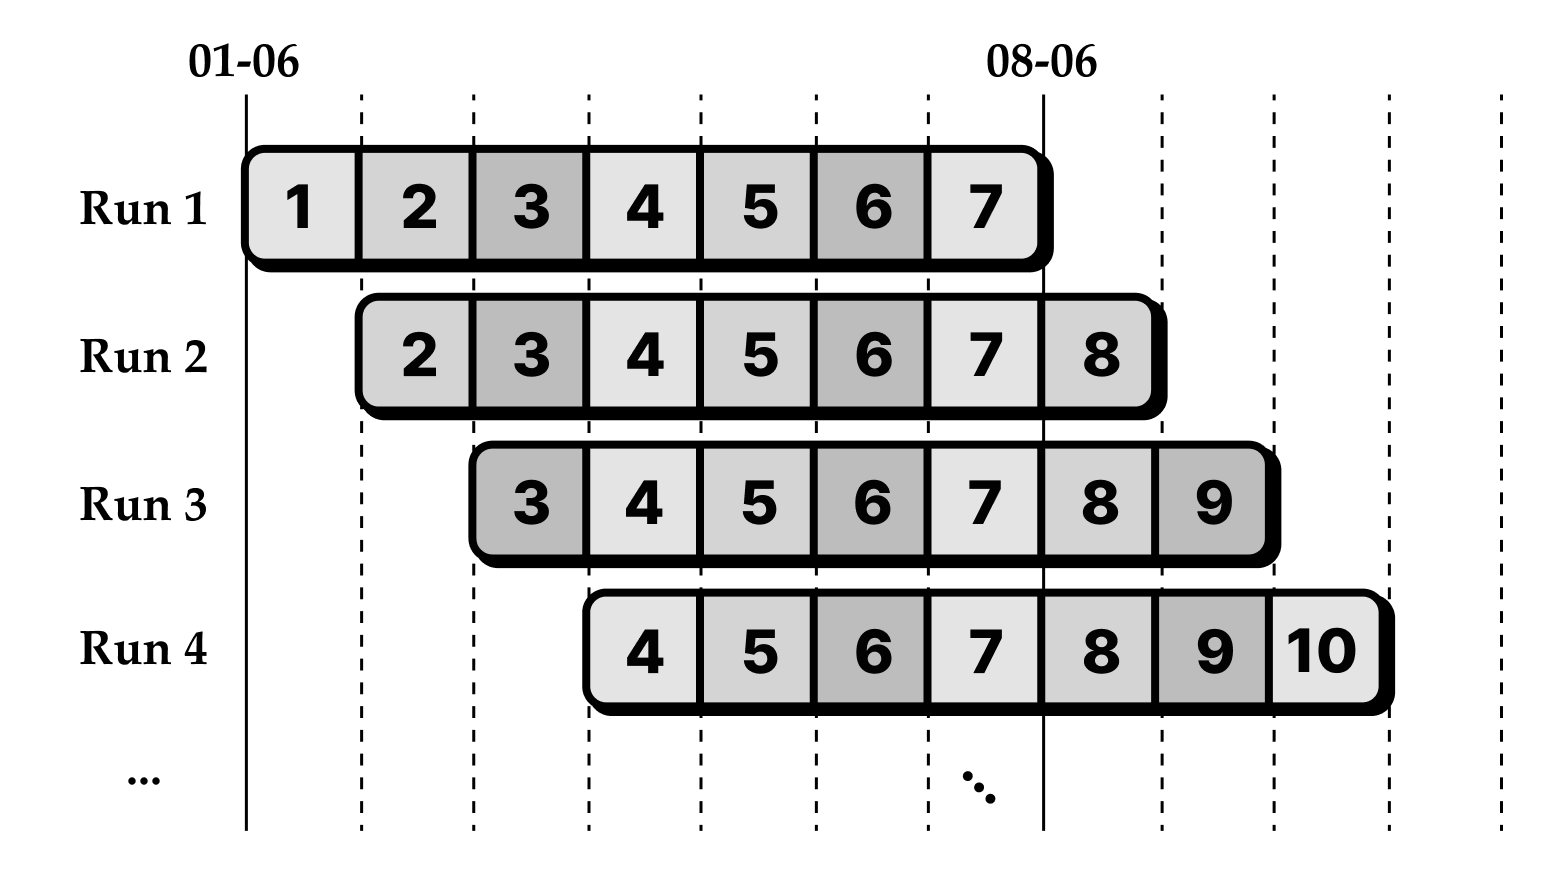
\includegraphics[width=11.65cm]{img/hs-grouping.png}
	\caption[Data grouping method used to combine data from overlapping simulation runs of HydroShoot.]{Data grouping method used to combine data from overlapping simulation runs of HydroShoot. Data with the same group number must stay together in a train, validation, or test set.}
	\label{fig:hydroshoot-grouping}
\end{figure}